\chapter{Fundamentação teórica} \label{chap:fundamentacao}

Este capítulo visa realizar uma abordagem de toda a fundamentação teórica e tecnológica necessária para o entendimento da solução proposta neste trabalho.

\section{\mhubcddl}

O \mhubcddl é uma composição de um \gateway (\mhub) e um \middleware de \iomt (\cddl). Enquanto o \mhub transforma o dispositivo \android em que está em execução em um \gateway \iot móvel, o \cddl funciona como \middleware provendo serviços locais e remotos de descoberta de provedores de serviços, processamento de eventos complexos, publicação e assinatura de dados e eventos com qualidade de serviço.

As seções seguintes abordarão cada um desses componentes separadamente.

\subsection{\mhub}

O \middleware \mhub pode ser definido, de acordo com \citeonline{talavera:et:al:2015}, como um serviço de \middleware de \iomt geral executado em um dispositivo móvel pessoal, responsável por descobrir e oportunisticamente conectar à uma miríade de \smartobjs acessíveis apenas através de tecnologias WPAN de curto alcance. Por estar envolvido com cenários de \iomt, este componenete de \software tem que lidar com situações que apresentam muito mais indeterminismo, devido à fatores como a menor garantia de disponibilidade de sensores e atuadores, confiabilidade reduzida, maior volatilidade em conexões, etc.

O \smartphone executando uma intância do \mhub, funciona como \gateway para \smartobjs, fornecendo acesso à internet para dispositivos que não podem se conectar. Outro recurso importante que pode ser explorado pelas aplicações é a habilidade de enriquecer os dados de sensores com dados de contexto obtidos dos sensores internos do \mhub.

Para que o \mhub tenha suporte à determinada tecnologia de comunicação, é necessário que um novo módulo seja implementado. Este módulo será responsável por gerenciar quaisquer operações que sejam necessárias para garantir o funcionamento desta tecnologia.

\subsubsection{\stwopa}

Para gerenciar a descoberta e conexão com dispositivos que trabalham com diferentes tecnologias de comunicação, além dos sensores internos do \smartphone, o \mhub utiliza o \textit{Short-range Sensing, Presence \& Actuation} (\stwopa), um protocolo que fornece uma \api comum para realizar a comunicação com diferentes tecnologias WPAN.

Implementado como um módulo na arquitetura do \middleware, o \stwopa define um conjunto de métodos e interfaces que os módulos responsáveis por determinada tecnologia de comunicação devem implementar. Isto permite que o \stwopa se comunique com todas as tecnologias WPAN suportadas, gerenciando-as, e assim fornece uma \api unificada para todas as camadas superiores da arquitetura que precisam se comunicar com tais tecnologias.

O \stwopa torna-se então um intermediador entre todas as tecnologias de comunicação específicas e os demais componenetes do \middleware. Dentre as funcionalidades---na forma de métodos e interfaces---que as tecnologias devem implementar para seu correto funcionamento no \middleware, destacam-se:

\begin{alineas}
	\item descoberta e conexão de \smartobjs;
	
	\item descoberta de serviços de cada \smartobjs;

	\item leitura e escrita de atributos de serviços (\textit{e.g.}, dados de sensores e comandos de atuadores);

	\item notificação de desconexão com \smartobjs.
\end{alineas}

É possível encontrar na \autoref{fig:technology-interface} a interface \techinterface definida pelo \stwopa que declara os métodos padrões que realizam as funcionalidades descritas, a qual todas as tecnologias devem implementar. Também é ilustrada a interface \techlistener que é implementada pela classe \stwopaservice---a implementação do \stwopa no \mhub.

\begin{figure}[htb]
	\centering
	\caption{\label{fig:technology-interface}Interface \techinterface}
	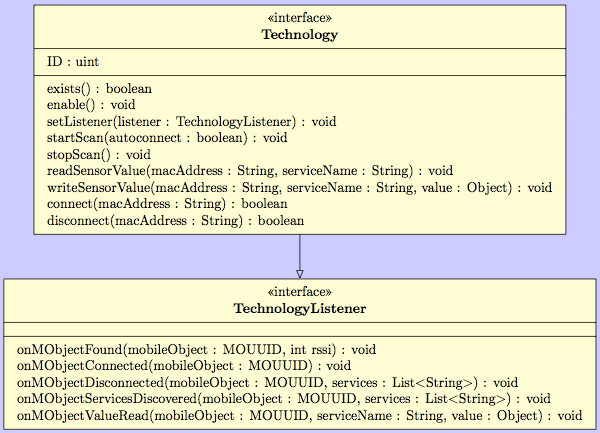
\includegraphics[scale=0.6]{img/technology-interface.png}
	\fonte{\citeonline[p. 125]{talavera:et:al:2015}}
\end{figure}

O \stwopaservice utiliza os métodos da interface \techinterface para gerenciar as tecnologias suportadas e, em particular, utiliza o método \texttt{setListener(\techlistener)} para se cadastrar como o \listener daquela tecnologia. Já as tecnologias utilizam os métodos da interface \techlistener para informar ao \stwopaservice a ocorrência de eventos com \smartobjs, como: descoberta, conexão, desconexão e leitura de dados de sensores.

O \mhub fornece diversos serviços que não serão tratados neste trabalho, dentre eles, destaca-se \cite{gomes:2017}:

\begin{alineas}
	\item \emph{protocolo de transcodificação}: 
		Os pacotes de dados recebidos dos sensores podem ter diferentes formatos e codificações.  Assim, o \mhub deve transcodificá-los e serializá-los, antes de transmiti-los. A transcodificação de dados é altamente dependente do tipo, marca e fabricante do sensor;
		
	\item \emph{caching de dados}: 
		A fim de otimizar a transmissão para a nuvem através da Internet móvel, o \mhub pode agrupar várias amostras de dados obtidas a partir de vários sensores próximos antes de enviá-las ao gateway em rajada única. Para isso, o \mhub armazena em cache as amostras de dados recebidas dos sensores;
		
	\item \emph{configuração e controle dos sensores}:
		Dependendo do tipo de sensor, o \mhub pode, eventualmente ou periodicamente, enviar comandos, definições de parâmetros ou requisições de consultas de dados através da WPAN para os sensores conectados;
		
	\item \emph{pré-processamento de dados do sensor}: 
		Antes de enviar os dados, pode ser necessário aplicar uma função de pré-processamento (e.g.  transcodificação, formatação, agregação, filtragem, ou comparação com leituras anteriores etc.).  Esse pré-processamento é feito no \mhub.
		
	\item \emph{carregamento dinâmico de módulos do sensor}: 
		Uma vez que não é possível ter módulos internos para todos os sensores que podem estar disponíveis a medida que o gateway se move, o \mhub oferece um mecanismo de implantação de módulo em tempo de execução e gerenciamento do ciclo de vida desses módulos;
		
	\item \emph{processamento nas pontas}: 
		O \mhub oferece mecanismos que permitem aos desenvolvedores de aplicações distribuírem as funcionalidades do seu código entre o dispositivo móvel e nodos da nuvem, movendo parte do processamento das informações de contexto para “as pontas” do sistema. A isso se dá o nome de In-Network Processing, uma técnica que ajuda a diminuir a quantidade de informações a ser transmitida para a nuvem, podendo melhorar a escalabilidade do sistema. O processamento ao qual esta funcionalidade se refere pode ser implementado em código Java convencional ou utilizando EPL Esper.
		
	\item \emph{processamento ciente de energia}: 
		Por meio de um componente de gerenciamento de energia, o \mhub monitora o nível da bateria do dispositivo móvel, disparando ações adaptativas que ajustam os comportamento dos seus serviços, de acordo com a disponibilidade de energia do dispositivo móvel. Por exemplo, a frequência de publicação dos dados por ser reduzida quando o nível da bateria está baixo (por exemplo, menor que 20\%).
\end{alineas}

A arquitetura do \middleware pode ser observada na \autoref{fig:m-hub-architecture}.

\begin{figure}[htb]
	\centering
	\caption{\label{fig:m-hub-architecture}Arquitetura do \mhub}
	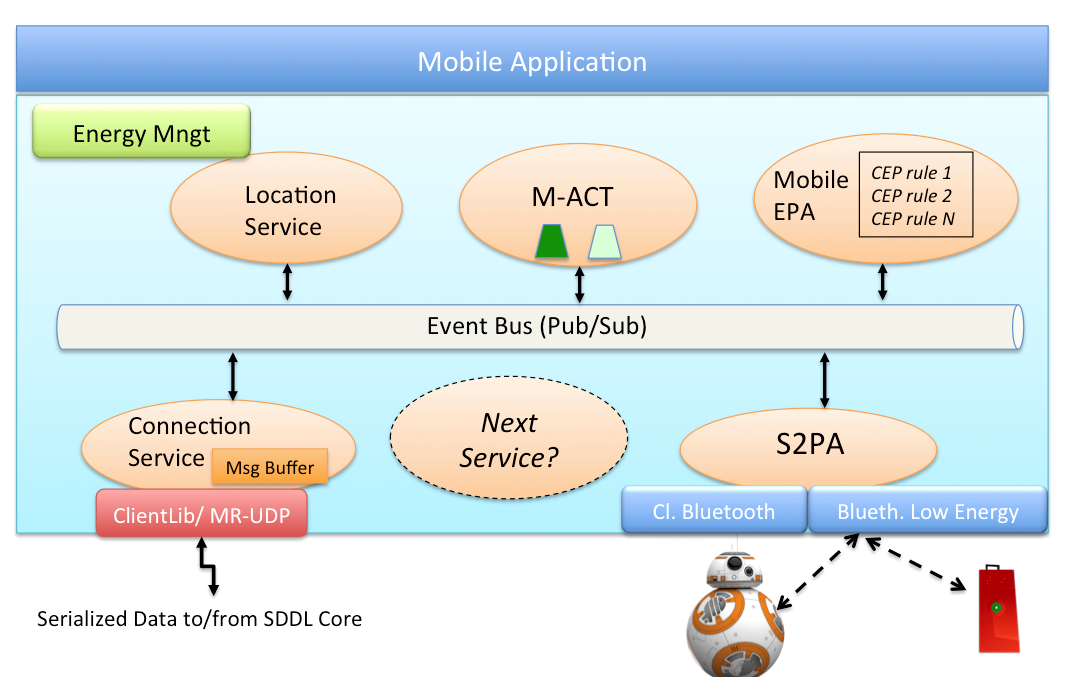
\includegraphics[scale=0.34]{img/m-hub-architecture.png}
	\fonte{\citeonline[p. 6]{endler:silva:2018}}
\end{figure}

\subsection{\cddl}

O \cddl é uma camada de distribuição de dados que provê mecanismos que permitem a especificação, controle e monitoramento de requisitos de qualidade de informação e do serviço de distribuição de dados \cite{gomes:2017}.

A interação entre produtores e consumidores de dados de contexto se dá através do modelo \pubsub com a utilização de \brokers, implementando uma comunicação ditribuída com o \mqtt. O \cddl também fornece um \ubroker que executa internamente no dispositivo móvel.

